\chapter{Task 3}
\begin{table}[hbt]
\centering
\caption{Reference Table 1}
\begin{tabular}{|l|l|l|l|l|} 
\hline
ID & \textbf{Description}            & \textbf{Duration} & \textbf{Predecessor} & \textbf{Required People}  \\ 
\hline
A  & Requirement survey server       & 3                 &                      & 2                         \\ 
\hline
B  & Requirements elicitation client & 2                 &                      & 2                         \\ 
\hline
C  & Implementation client           & 6                 & B                    & 1                         \\ 
\hline
D  & Implementation server           & 3                 & A                    & 1                         \\ 
\hline
E  & Recruit test subjects          & 3                 &                      & 1                         \\ 
\hline
F  & Procure server hardware         & 2                 &                      & 2                         \\ 
\hline
G  & User tests and improvements~    & 4                 & C, E                 & 2                         \\ 
\hline
H  & Load test on real hardware      & 4                 & D, F                 & 1                         \\ 
\hline
I  & Automate deploymen              & 2                 & H                    & 1                         \\ 
\hline
J  & Going live                      & 3                 & G,I                  & 1                         \\
\hline
\end{tabular}
\end{table}
% \usepackage{tabularray}
\begin{table}[hbt]
\centering
\caption{Reference Table 2}
\begin{tblr}{
  row{1} = {c},
  row{2} = {c},
  cell{2}{1} = {c=3}{},
  cell{3}{1} = {c},
  cell{3}{3} = {c},
  hlines,
  vlines,
}
Earliest Start & Duration    & Earliest Finish \\
Activity Label &             &                 \\
Latest Start   & Slack/Float & Latest Finish   
\end{tblr}
\end{table}
\newpage

\begin{parlist}
	\item Solution: 
	\begin{figure}[hbt]
	\centering
  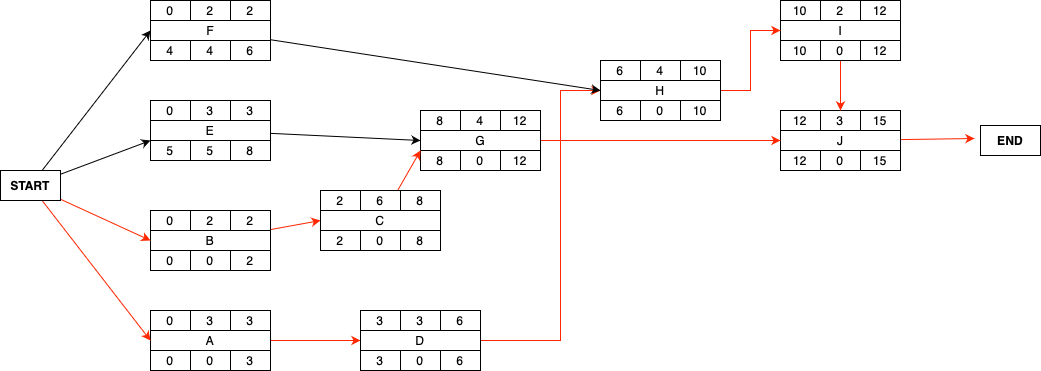
\includegraphics[width=1.4\textwidth]{Immagini/ND.png}
	  \caption{Task 1.a and 1.c}
\end{figure}
\\
Earliest start = Latest start form previous activity (going from left to right)\\
Last finish = Earliest finish from previous activity (going from right to left)\\
Latest start = Latest finish - Duration\\
Slack = ES -LS or EF - LF\\
Critical path is formed when activities have 0 slack. (in red) \cite{CriticalPath}

	\item Solution:
\begin{figure}[hbt]
	\centering
  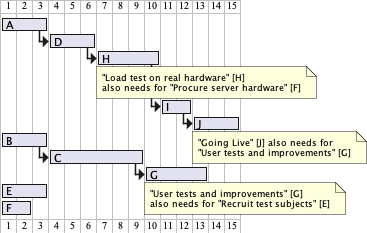
\includegraphics[width=0.85\textwidth]{Immagini/ganntChart.png}
  \caption{GanntChart}
\end{figure}
\end{parlist}